% !TEX root = Hogwarts_1347.tex

\chapter{The Castle}

Thomas stepped down from the carriage onto flagstone. The ground was old and uneven, worn smooth in places by centuries of feet, and after the long, swaying hours on the road it felt impossibly, almost aggressively solid beneath his boots. Colum dropped down beside him, steadied himself with a hand on the carriage frame, and looked up.

The castle filled the sky.

From the glen, it had been a silhouette --- towers and turrets and high curtain walls, impressive but reducible to a shape against the clouds. Here, at the foot of its own rock, the scale defeated the eye. The walls rose sheer from the stone outcrop, their surfaces a patchwork of grey and darker grey where rain and lichen had worked the masonry over centuries. Buttresses the size of houses braced the lower courses. Above them, towers climbed at heights that should not have held, their windows catching the afternoon light in scattered points that moved as the clouds shifted. Gargoyles crouched along the parapets --- dozens of them, each different, each watching a different quarter of the sky with the fixed, humourless attention of sentries who had not been relieved in four hundred years.

A broad stone stairwell led from the courtyard to the main entrance --- a pair of heavy oak doors, iron-studded and tall enough to admit a mounted knight, set deep within a pointed arch. Students were already climbing the steps, their trunks floating or dragged behind them.

Cecile and Celine emerged from the carriage behind them. Celine stood for a moment, her head tilted back, her lips slightly parted, taking in the full vertical reach of the nearest tower. Cecile placed a hand on her sister's shoulder --- gently, briefly --- and then began walking toward the stairs with the purposeful stride, returning to a place she knew.

Thomas did not follow immediately. He turned instead to take in the broader scene.

The courtyard was alive with arrival. From the direction of Hogsmeade, a steady procession of figures descended through the air on broomsticks --- older students, by the look of them, their landings practised and unhurried, their trunks roped to their backs or levitated alongside. A few staff members arrived the same way, distinguishable by their heavier robes and the particular, unhurried authority with which they touched down. One witch landed on the far side of the courtyard carrying what appeared to be an enormous potted shrub under one arm and a stack of leather-bound folios under the other, dismounting with the ease of someone stepping off a low wall.

It was a scene of controlled chaos --- the ordinary, annual machinery of a school reassembling itself after a summer apart.

Then his eye found the patch of grass.

It lay perhaps twenty metres from the foot of the stairwell, a level stretch of turf running along the base of the castle's eastern wall. Two figures occupied it, and the space around them was conspicuously empty --- not because anyone had been told to keep their distance, but because the nature of what was happening there made distance the only sensible response.

A man and a girl were training in combat --- defence techniques, by the look of it.

The man was tall and lean, his stance low, his weight distributed with the particular economy of someone who had spent years learning exactly how much movement was necessary and how much was waste. He was in his late forties, perhaps older --- his dark hair, cut short, was already heavily threaded with white, and the lines on his face carried the deep-set quality of marks that had been earned rather than aged into. His eyes were watchful in a way that went beyond attention; they moved with the constant, restless sweep of a man who had trained himself never to stop scanning.

The girl opposite him was slight, her long dark hair pulled back into a single, practical braid that hung between her shoulder blades. Her skin was very pale; freckles dusted the bridge of her nose and her cheekbones. She had the most piercing blue eyes --- not dark or sharp, but soft and luminous, hazy like the blue of a summer sky --- with pinpoint pupils.

She held her wand with an ease that did not belong to her age.

Both wore padded gambesons --- the quilted, close-fitting garments that Thomas recognised from illustrations in his Defence texts, designed to absorb the residual force of deflected spells. The man's was a worn, creamy white with green edging along the front opening, collar, and cuffs, and a small Slytherin crest embroidered over the left breast. The garment showed the unmistakable signs of extensive use and many repairs --- patches of newer fabric where old burns had been cut away, a long seam along the ribs that had been resewn with heavier thread. It was the gambeson of a man who trained often and kept what worked --- but the depth of its wear suggested it had seen more than mere training.

The girl's was black with orange edging, cut tighter to her smaller frame, and conspicuously newer --- the colours still vivid, the stitching clean, the padding still full. It bore no house emblem.

The man opened.

\enquote{\textit{Stupefy}.}

The red bolt crossed the distance between them in less than a heartbeat. The girl sidestepped it --- not by a foot, not by a generous margin, but by a hand's width, the spell passing close enough to disturb the loose strands of hair at her temple. The economy of it was striking. She had moved exactly as much as she needed to and not a fraction more, as though she had measured the trajectory of the spell in the instant it left his wand and calculated the minimum displacement required to survive it.

She returned fire before the red light had finished dying in the air behind her.

\enquote{\textit{Expelliarmus}.}

He blocked it. His shielding spell was quick and textbook --- a sharp, practised flick that sent her disarming charm scattering into white fragments. She blocked his counter with the same clean efficiency. He sent another. She deflected, adjusted her footing, and fired back.

The exchange accelerated.

The spells began to overlap --- red, white, red --- each one arriving faster than the last, the interval between cast and counter compressing until the individual incantations blurred into a continuous, percussive rhythm. The cracks of impact echoed off the stone wall behind them, sharp and flat, like the reports of a whip. Thomas could see the effort in both of them now --- the man's jaw set, his wand arm moving in tight, controlled arcs; the girl's braid swinging with each pivot, her feet adjusting on the grass with small, quick steps that kept her balanced and mobile.

It was a lesson --- fast, fluid, but not dangerous. A drill between two people who had done this many, many times before.

Then the man sent a disarming charm that was harder than the rest, maybe a bit too hard, he thought to himself.

Thomas saw it in the man's shoulder --- the slight, additional rotation, the extra half-inch of extension in the follow-through that loaded more force into the spell than any of the previous exchanges. It crossed the grass like a thrown stone. The girl's shield caught it --- her wand was already in position, the defence technically sound --- but the force of the impact travelled through the charm and into her arm, pushing her back half a step. Her rear foot slid on the wet grass. Her balance broke.

Instead of recovering, she slashed her wand in a sharp, vicious diagonal and spoke two words.

\enquote{\textit{Sanguinem Scinde}.}

The man's wand hand opened from within. The skin parted in a clean, bright line across the palm --- not from impact, not from any force that had struck him from outside, but as though the blood itself had chosen to leave. The wound was precise and bloodless for a single, suspended instant before the red welled up and ran freely between his fingers. His wand fell to the grass.

The girl lowered her wand and stood still, breathing hard.

The courtyard had gone very quiet.

The man bent, retrieved his wand with his uninjured hand, and pressed its tip against the split palm. The skin drew together and closed cleanly, the blood ceasing as though a tap had been shut. He flexed his fingers once, then again, testing the repair with the methodical patience of a man who had mended himself many times before and understood the importance of checking the work. He did not look up while he did this.

When he spoke, his voice carried across the field with a clarity that made several students near the carriages go still.

\enquote{Laura.}

He was still looking at his hand, turning it over, examining the line where the wound had been. But his voice had a tightness to it that had nothing to do with the injury.

\enquote{Good wizards are above certain spells.} He looked up. His eyes locked onto hers, and his face held a frustration and an anger that Thomas recognised --- the kind that can only come from someone who deeply loves and cares. \enquote{The best wizards have no need for such spells. None! Do you hear me?}

For a moment, Thomas thought she might argue. Her jaw tightened, and her chin lifted a fraction --- the smallest, most instinctive gesture of defiance. Then something in his expression reached her, or something in her own chest answered it, and the defiance collapsed. Her lip pressed tight against the upper, and her eyes filled.

The man crossed the distance between them in three strides, pulled her into his arms, and kissed the top of her dark hair. She pressed her face against the white gambeson, her small hands gripping the quilted fabric at his sides. He held her. The arm that had been wounded wrapped around her shoulders without hesitation, as though the hand had already forgotten what it had cost.

They stood like that for several seconds, the girl's face hidden, the man's chin resting on the crown of her head, his eyes fixed on something far beyond the courtyard wall. Then he released her, placed both hands on her shoulders, and said something too quiet to carry.

She nodded once.

\section*{The crib}

Thomas was still watching when a hand landed on his shoulder with enough force to suggest its owner had not entirely mastered the art of measured physical contact.

Baldwin came bounding around from the back of a carriage, half-running, half-jumping, his spectacles slightly askew, his face flushed with the unmistakable expression of an eleven-year-old boy who had just seen something he had only ever read about.

\enquote{Merlin's \textit{beard},} Baldwin breathed, gripping Thomas's arm. \enquote{Is that ---}

\enquote{Professor Hugh Li\ldots{}} Cecile said, approaching from behind them. Her voice was calm, but her eyes had not left the pair on the grass.

\enquote{Laura Orwell,} Baldwin interrupted her.

Thomas looked between them. \enquote{Who?}

Philippa, who had just appeared beside them with the quiet inevitability of someone who never missed a conversation worth hearing, gave Thomas a look of undisguised disbelief.

\enquote{Have you been living under a rock? She's Hogwarts' biggest mystery since the Chamber of Secrets.}

\enquote{Chamber of what now?} said Thomas.

\enquote{Never mind.} Baldwin's hand was still on Thomas's arm. He was practically vibrating. \enquote{Eleven years ago, to this very day, the four ships of the Hogwarts convoy entered the loch. The \textit{Melusine} was still under construction in the shipyard, so there were only four --- the \textit{Mermaid}, the \textit{Siren}, the \textit{Ceasg}, and the \textit{Merrow}. The port had been assembled, everything was normal, and then ---} He faltered, not from forgetting, but from the sheer pressure of wanting to say everything at once.

Philippa picked up the thread with the easy authority of someone who had heard the story from more sources. \enquote{A fifth ship appeared drifting slowly towards the port. A full-sized hulk, larger than any of the sisters and darker in colour.}

\enquote{They boarded it,} Cecile continued, her voice lower. She had heard this from older students who had heard it from older students still, and the story had acquired the particular, reverent weight of a tale told many times in common rooms after dark. \enquote{It was in pristine condition, no damage, no marks on the hull to suggest what had happened or where it had been. No crew either, no passengers, no cargo, no log. The galley was cold. The water barrels were full. The rigging was set as though someone had just finished trimming the sails and then simply\ldots{} ceased to exist.}

\enquote{Empty,} Philippa said. \enquote{Completely empty. Except ---}

\enquote{Except for a baby,} Baldwin said, unable to contain himself any longer. \enquote{A newborn girl, alive and healthy, wrapped in a clean blanket, lying in a beautiful crib in one of the cabins of the sterncastle. The name \textit{Laura Orwell} was carved into the wood on one side. Nothing else. No letter, no seal, no indication of who had placed her there or why.}

\enquote{The Wizards' Council launched an investigation,} Philippa added. \enquote{Every wizarding and Muggle ship on the western seaboard was accounted for. A few wrecks were checked --- none matched the design. The hull itself resisted every charm they cast to trace its origin. The crib was examined by three separate experts. Nothing.}

\enquote{Eleven years,} Baldwin said, shaking his head slowly, \enquote{and not a single answer.}

\enquote{By the Headmaster's request, her guardianship was assigned to Professor Ligier,} Philippa said. \enquote{He grew fond of her and adopted her shortly after.}

Baldwin nodded. \enquote{She was raised within the castle walls. Learned to walk in its corridors, grew up among the ghosts and the portraits and the shifting staircases.} He paused, adjusting his spectacles. \enquote{Hogwarts is not her school. It is, and has always been, her home.}

Ligier and Laura reached the heavy oak door at the top of the stairs. He pushed it open with his free hand and guided her through. The door swung shut behind them with a low, resonant thud that carried down the steps and across the courtyard. They did not look back at the carriages. They did not acknowledge the arriving students.

The group stood in silence for a moment, watching the closed door.

\enquote{But who left her there?} Celine asked.

Her voice was soft, carrying the particular quality of a question asked not because the speaker expected an answer, but because the absence of one felt unbearable.

Baldwin looked at the heavy oak door at the top of the stairs, now shut and still, as though it had never opened.

\enquote{Nobody knows.}








\section*{The Mirror}
 
The interior courtyard was one of the quieter spaces of Hogwarts, enclosed on all sides by pale walls and narrow arched corridors. The masonry was clean and severe rather than ancient, recently raised by wizarding hands but already bearing the marks of hard weather and hurried passage. In one corner stood a single oak tree, deliberately planted, its branches spreading just wide enough to cast shade across the flagstones and soften the echo of footsteps.
 
Students clustered everywhere: some whispering in hurried Latin, others laughing too loudly, a few standing apart with rigid backs and hands clenched around borrowed trunks or sleeves. It was the sort of noise made by children pretending not to be anxious.
 
Celine was still in one of the corridors that opened onto the courtyard, walking slowly toward the light. She held the mirror carefully, as though afraid that even her breath might disturb it. The glass shimmered faintly, catching more than light --- movement, distance, warmth.
 
Her father's face wavered into focus.
 
\enquote{Are you warm enough?} he asked, his voice tinny but warm. Behind him, the wooden masts and salt-stained rigging of a ship swayed against a pale sky.
 
\enquote{I'm fine,} Celine said quickly. \enquote{Truly. The castle is\ldots{} huge. It is a forest of stone towers and high bridges, larger than any cathedral I could have imagined.}
 
He smiled, though worry still clung to the corners of his eyes. \enquote{Your sister?}
 
\enquote{Nearby,} Celine said, glancing across the courtyard. Cecile was speaking animatedly with a tall girl, her hands moving as if she was already in a classroom explaining something important.
 
Her father nodded. \enquote{Good.} He hesitated, then added, more firmly, \enquote{Listen to me. Whatever house they put you in, you won't be alone. You'll always have your sister. And Philippa, she's sharp. Stay close to her.}
 
Celine nodded, blinking. \enquote{I will.}
 
She had just begun to lift the mirror closer, as if to imprint his face into memory, when a shadow fell across the glass.
 
\enquote{Well, that's interesting.}
 
The voice was sharp, amused in a way that made her stomach tighten. Hector Hawthorne stood there, a boy with an air of mocking confidence. Before Celine could react, his hand darted forward and seized the mirror by its edge.
 
\enquote{Hey ---!} Celine cried, lunging, but Hector was already moving.
 
He was quick, light on his feet, darting backward with a laugh as he turned the mirror over in his hands. The image of her father flickered wildly, then vanished into a blank shimmer.
 
\enquote{What's this?} Hector said, loud enough that several nearby students turned. \enquote{Talking to people already? Didn't know we were allowed visitors.}
 
\enquote{Give it back,} Celine said, her voice trembling despite herself. \enquote{It's not yours.}
 
He ignored her, craning his neck as though trying to peer deeper into the glass. \enquote{That wasn't anyone from here,} he said. \enquote{No robes. No wand. Funny way of speaking, too.}
 
A few students laughed. Others watched silently.
 
Celine stepped forward again, her hands half-raised. \enquote{Please.}
 
Hector's smile widened. \enquote{Please,} he echoed. \enquote{Did he teach you magic too\ldots{} or is he a muggle?}
 
Cecile's voice cut across the courtyard. \enquote{Leave her alone!}
 
She was already moving, pushing past two older boys, her face flushed with anger. But Hector Hawthorne was faster. He spun on his heel and bolted toward the oak tree.
 
\enquote{Catch me if you want it back,} Hector called, already scrambling up the low stone border and grabbing the lowest branch.
 
Celine stood frozen, heart pounding, staring upward as he climbed. The mirror glinted between his fingers.

That was when Thomas decided to act. He had been standing a step behind Colum, quiet, observant, his posture loose enough to seem almost uninterested. When he moved, it was without haste or drama. His left hand lifted slightly at his side, fingers straight, and several pale strands of his own hair were already looped around them, tangled there as if by habit rather than intention. His eyes found the back of Colum's wand hand --- and held.

Colum, wand already in hand from nervous habit, stiffened. His arm jerked upward, sharp and sudden, as if seized by an invisible string. His wrist turned, his elbow locked, and the wand's tip snapped into line with Hector in the tree. Colum felt the pull travel through his shoulder and down to his fingers --- a cold, precise pressure that moved his joints with an authority that was not his own.

\enquote{Wait ---!} Colum said, startled, his fingers tightening uselessly around a wand that had nothing to do with what happened next.

A flash of light lanced forward from behind Colum and crossed the courtyard in a flat, bright line. It passed so close to the tip of the outstretched wand that the difference was invisible to anyone watching from the front --- which was everyone. From where the courtyard stood, the spell had come from Colum's wand. From where Thomas stood --- one step behind, his left hand low at his side, the strands still wound tight across his knuckles --- it had not.
  
It wasn't violent, not exactly. It was quick and precise, like a decision made too fast to reconsider.
 
Hector yelped as an unseen force struck him squarely in the chest. He flew backward, spinning twice before landing hard on the stone with a thud that echoed through the courtyard.
 
The mirror hit the ground a heartbeat later.
 
The sound it made --- sharp, brittle, final --- cut through everything.
 
Silence fell.
 
Celine stared at the ground, her breath caught somewhere between her ribs and her throat. The mirror lay in pieces --- four of them --- its shimmer gone, the surface dull and lifeless.
 
Cecile reached her at last, wrapping an arm around her shoulders. \enquote{It's all right,} she said fiercely, though her eyes were fixed on the broken glass. \enquote{It's all right.}
 
Hector sat up slowly, groaning, his bravado evaporated. A few students murmured. Others stepped back.
 
All eyes turned to Colum Douglas, whose face had gone pale.
 
\enquote{I ---} he began. \enquote{I didn't ---}
 
But Cecile was already turning to Colum. She seized his sleeve, eyes bright with gratitude. \enquote{\textit{Merci}, thank you,} she said, and before he could react, she leaned forward and kissed his cheek.
 
His ears turned red instantly.
 
From the edge of the courtyard, Professor Magnus Grim had been watching.
 
He stepped forward now, his long coat whispering against the stone. He did not raise his voice. He did not scold. He simply looked down at the boy on the ground.
 
\enquote{Mr. Hawthorne,} he said calmly. \enquote{Hogwarts does not take well to bullies.}
 
Hector swallowed and looked away.
 
As Grim straightened, his gaze flicked --- not to Colum, not to Cecile --- but briefly, deliberately, to Thomas. Thomas stood where he had been a moment before --- a step behind Colum, his left hand now resting loosely at his side, the pale strands of hair no longer visible between his fingers. His expression was carefully, perfectly blank. One eye closed and opened again, so quick it might have been dismissed as dust or strain. But it was not.
 
Professor Grim, Thomas, and Colum knelt and collected the mirror pieces.
 
Grim rose, holding the pieces he had taken. He plucked a small white daisy growing improbably between the stones nearby and tucked it into his sleeve.
 
\enquote{Miss Celine. Miss Cecile. You two as well,} he said, looking to Colum and then to Thomas, whose expression remained carefully blank. \enquote{Come with me.} He turned and walked away without another word, evidently certain they would follow. They did.
 
Behind them, the courtyard slowly began to breathe again --- but something had shifted, unnoticed yet irreversible.
 
\section*{The Workshop}
 
The Fournier sisters, Colum and Thomas followed Professor Magnus Grim in silence. Philippa, who had not been explicitly invited but possessed the distinct talent of appearing as though she belonged, fell into step beside them. Grim did not object.
 
They wound through a labyrinth of stone corridors until they reached a small, unassuming wooden door set deep within the castle's spine. Professor Grim halted. He raised his wand, tracing a silent glyph in the air. The iron lock gave a sharp, satisfying click, and the door swung inward.
 
With a flick of his wrist, the heavy velvet curtains at the far end of the room swept open, allowing the Highland light to flood the dusty space. With another flick, the oil lamps mounted on the stone walls flared to life, their warm yellow glow mixing with the daylight to create an amber haze. The room was part study, part workshop, filled with ticking instruments and the smell of ozone and new parchment.
 
Grim ushered them inside and, with a wave of his wand, pushed two high-backed chairs forward for Celine and Cecile. The door clicked shut behind them, sealing out the noise of the castle.
 
\enquote{The fragments,} Grim said, extending a hand.
 
He placed the two shards he had gathered onto his workbench. Colum and Thomas stepped forward, placing their own pieces beside them.
 
Grim stood over the broken glass. He flicked his wand and muttered, \enquote{\textit{Revelio}.}
 
Nothing happened. The glass remained dull and inert.
 
Grim hummed, unimpressed. He turned to the cold fireplace, summoning a generous handful of grey wood ash into his palm. He blew the ash into the air above the table, where it hung suspended in a gravity-defying cloud.
 
\enquote{\textit{Diagnosce et manifestare},} he intoned.
 
Immediately, the swirling ash coalesced. It darkened and amalgamated, forming complex geometric shapes and thin, ghostly strings in the air above the mirror pieces. Some of the shapes were twisted and deformed; many of the connecting strings snapped and whipped in the air, seeking anchors that no longer existed.
 
\enquote{Interesting,} Grim murmured, leaning closer, his eyes reflecting the floating ash. \enquote{Intriguing\ldots{} oh, unfortunate.}
 
He opened a drawer and levitated a thin filament of pure gold. With a subtle twist of his wand, the metal disintegrated into a fine, shimmering powder. He directed it into the suspended ash, mixing the gold with the grey.
 
Then, he began the surgery.
 
With precise movements of his wand, Grim distanced the four mirror fragments from one another. He slashed his wand through the air, rupturing the ghostly strings that still tried to connect the shapes above the different pieces. The snap of the breaking magic was audible, like the plucking of a taut violin string.
 
For each isolated shard, he began to weave. He reshaped the ash and gold above each piece, tying the loose ends back onto themselves, creating four self-contained loops of magic.
 
He lowered his wand. The cloud of ash and gold dust glowed with a sudden heat, then rained down, melting into the glass surface.
 
At that moment, the surface of the mirrors rippled. Grim picked up one shard, holding it close to his face. Instantly, the image of his eye --- magnified and inquiring --- appeared not in the piece he held, but on the surface of the three shards still lying on the table.
 
Grim nodded, satisfied. He went to place the shard back down, but his thumb grazed a jagged edge.
 
\enquote{Ouch.}
 
A bead of bright red blood welled on his finger. Grim frowned at it, pressed his wand tip briefly to the cut --- sealing it --- and wiped the smear of blood from the glass with his sleeve before it could settle into the enchantment.
 
He turned back to the drawer. Two metallic filaments floated out --- one of reddish copper, the other of dull tin. Under the heat of his silent will, portions of the metals liquified, swirling together in mid-air to fuse into a glowing, golden-brown bronze.
 
The alloy stretched out like taffy, forming a thin, flat bar. Grim sliced the bar into four sections. With delicate care, he wrapped the warm bronze around the jagged perimeter of the first shard, the metal cooling and hardening instantly to form a protective rim. He repeated this for the other three.
 
The work was not done. With the tip of his wand, he carved into the cooling bronze, etching tiny, intricate petals and vines. He levitated a final thread of silver, melting it into the grooves he had just carved. The silver shone stark and beautiful against the bronze.
 
Grim stepped back and flicked his wand over the finished pieces.
 
\enquote{\textit{Desiste}.}
 
The reflections on the mirrors vanished, returning to normal glass.
 
He flicked his wand again. \enquote{\textit{Reflecte}.}
 
The surface shimmered, and once again, the shards linked, each reflecting the view of the others.
 
Professor Grim gathered the four artifacts and turned to the students. His expression was serious, the earlier flash of pain forgotten.
 
\enquote{As is often the case with magical artifacts,} he said, his voice dropping to a lecture tone, \enquote{especially the complex ones, the original vessel could not be fixed. The enchantment that bound it is severed.}
 
He held out the pieces.
 
\enquote{However,} he continued, \enquote{just because something is broken, it doesn't mean its parts can't be repurposed. A shattered whole may yet birth new instruments.}
 
He placed the four framed mirrors into Celine's hands.
 
Celine looked down at them. They were no longer a single window to her home, but something new. Something shared.
 
She kept one for herself. She handed the second to Cecile. She turned and pressed the third into Philippa's hand. Finally, she stepped toward Colum and offered him the last one.

Colum took it, his thumb brushing the silver-inlaid bronze, the glass cool against his palm.
 
Professor Grim dusted the remaining ash from his palms and glanced toward the heavy hourglass sitting amidst the clutter of his desk. The sand was running dangerously low.
 
\enquote{Now,} he said, his tone shifting from that of an artisan back to a master of the school. \enquote{We had best secure those and make haste to the Great Hall. The Sorting Ceremony is imminent, and it would not do to be absent before the proceedings even commence.}
 
He ushered them toward the door, extinguishing the oil lamps with a sweeping wave of his hand as they passed, plunging the room back into shadows.
 
\enquote{Come,} he commanded, opening the door for them.
 
\section*{The Sorting Hat}
 
The hall was quieter than Thomas had expected. It was not a void of sound, but a heavy, expectant restraint, as if the severe stone walls were leaning in to listen. Above, the ceiling whispered faintly with the drift of candle-smoke and the low thrum of magic.
 
Professor Magnus Grim stood beside the three-legged stool, utterly still, his long dark coat falling to the stone floor. As the Head of Gryffindor, he held the weathered Hat with a quiet reverence, his sharp eyes scanning the rows of new faces.
 
One by one, names were called.

%\bigskip
\vspace{1.5\baselineskip}

\enquote{Celine Fournier,} professor Grim called, nailing the French pronunciation, Celine observed.

Celine walked forward with a small, hesitant step. There was an unmistakable innocence in the way she looked at the Great Hall --- a trusting curiosity that seemed untouched by the cynicism of the older students. As she climbed onto the stool, Professor Grim lowered the Hat over her eyes. It slipped low, almost touching the bridge of her nose.
 
\enquote{Ah,} a voice whispered in her mind, gentle and resonant. \enquote{So open. A heart that expects the best of the world, isn't it? Such a rare, trusting thing.}
 
Celine stiffened, but she did not pull away.
 
\enquote{Kindness first,} the Hat murmured. \enquote{Always kindness. A heart that would rather be hurt than become hard\ldots{}}
 
A pause stretched out.
 
\enquote{Hufflepuff would keep you safe. It would cherish that innocence. But you would not stay safe, even if I asked you to. When the time comes, your trust will become your shield, and you will step forward while others hide. Yes\ldots{} I see it now. Not boldness --- but bravery.}
 
\enquote{GRYFFINDOR!}

The table erupted. Celine slid off the stool, dazed and smiling, and Cecile's hands were already on her shoulders as she reached the bench.
 
Other names were called. Some were met with roaring cheers, others with polite applause, each student finding their table and their place.

%\bigskip
\vspace{1.5\baselineskip}

\enquote{Philippa Laskaris.}

Philippa sat with a perfect, icy composure. She didn't look at the Hat; she looked at the people. She mapped the faces of the professors and the cliques forming at the tables, already gauging the social architecture of the school. Philippa might not have known every secret of the castle yet, but she already knew exactly who to watch to find them. Professor Grim placed the Hat upon her head.
 
\enquote{Oh, you see the strings, don't you?} the Hat hummed thoughtfully. \enquote{It is not just about what is known, but who knows it. You are a weaver of connections. You know who speaks to whom, and exactly which hand to hold to open a locked door.}
 
Philippa's chin lifted slightly.
 
\enquote{Ravenclaw would value your mind, but you do not care for books as much as you care for the people who write them. Slytherin would teach you to rule those connections. But there is a fire in you that refuses to remain in the shadows. You want the world to see your work.}
 
\enquote{GRYFFINDOR!}
 
Philippa smiled --- a sharp, knowing expression --- as if she had already decided this was the most advantageous outcome.
 
The ceremony continued --- name after name, the Hat deliberating briefly with some, longer with others, the four tables filling steadily.

%\bigskip
\vspace{1.5\baselineskip}

\enquote{Hector Hawthorne.}

When Hector's name was called, he walked to the stool with a swagger. Professor Grim's expression remained unreadable as he lowered the Hat.
 
\enquote{Pride of lineage and a sharp eye for leverage,} the Hat said with cold clarity. \enquote{You seek the high ground, Hawthorne. You seek the company of those who understand that power is a currency and everything is transactional.}
 
Hector's jaw tightened. He didn't look afraid; he looked hungry.
 
\enquote{You will find your kin among those who sharpen themselves against the world.}
 
\enquote{SLYTHERIN!}
 
Hector stood and headed for the green-draped table, where several older students nodded to him with narrow-eyed approval.
 
More names followed. The list was long --- students from every corner of the British Isles and beyond --- and the hall settled into the rhythm of the ceremony, each sorting met with its own brief eruption before the quiet returned.

%\bigskip
\vspace{1.5\baselineskip}

\enquote{Thomas Blackwood.}

When Thomas took his seat, Professor Grim lowered the Hat. Then, everything stopped.
 
The Hat did not speak. It did not shout. It began to mutter, a low, rhythmic grumble that only Thomas could truly hear, though the entire hall could see the brim twitching and folding.
 
One minute passed. Then two. The restless shifting of the students began to die down, replaced by a heavy, confused silence.
 
\enquote{Cecile? Why is it taking so long? Is something wrong?} Celine leaned closer to her sister, her voice a tiny whisper.
 
Cecile was staring at Thomas, her eyes wide with a mixture of awe and fear. \enquote{It's a Hatstall,} she breathed, her voice trembling. \enquote{I heard about this\ldots{} it's very, very rare. Once in a generation. It happens when the Hat finds a mind so complex that it cannot choose.}
 
Five minutes passed. Thomas sat like a statue, his knuckles white where he gripped the stool. The Hat's murmuring grew louder, a frantic, debating sound.
 
\enquote{Difficult\ldots{} so very difficult. There is power here --- raw, instinctive, undisciplined. With discipline you could command things. You could shatter them too, boy.}
 
Thomas did not move. He did not want to command anything. He just wanted the Hat to finish.
 
\enquote{Slytherin would give that power a purpose. It would hone that instinct into a weapon. You could be great --- recognised across the kingdoms.} The Hat groaned, the leather twisting. \enquote{But you\ldots{} you do not want the glory, do you? You don't seek the applause. You just do what is right, simply because it is right. A dangerous, unyielding honesty.}
 
Eight minutes. Ten. The silence in the hall was now absolute, broken only by the flickering of the candles. Even Professor Grim's expression had tightened.
 
\enquote{Power like yours belongs in Slytherin to be mastered,} the Hat whispered, sounding almost exhausted. \enquote{But a soul like yours\ldots{} it belongs to the fight. You would rather be a shield than a crown.}
 
Finally, the Hat's brim opened wide.
 
\enquote{GRYFFINDOR!}
 
The roar that followed was less like a cheer and more like a release of built-up pressure. Thomas stood up slowly, his face still a mask of neutrality, though his heart was racing. He caught Professor Grim's eye; the Professor gave a single, almost imperceptible nod of respect.
 
The ceremony resumed. After the extraordinary length of Thomas's sorting, each subsequent name felt brisk by comparison --- the Hat settling quickly, the tables responding, the list steadily shortening.

%\bigskip
\vspace{1.5\baselineskip}

\enquote{Edmund Varre.}

A boy rose from the benches and walked to the stool with a measured, unhurried stride. His appearance was immaculate --- an overcoat of dark wool, elegantly cut and cinched tight at the waist, falling over perfectly ironed trousers and shoes polished to a mirror shine. He sat, crossed one ankle behind the other, and folded his hands in his lap. Professor Grim lowered the Hat.

It barely touched his head.

\enquote{Easy... so very easy. There is only one house your heart ever considered. SLYTHERIN!}

Edmund stood, and in a single, rehearsed motion, unbuttoned his overcoat. Beneath it, he was already wearing the full Slytherin uniform --- the emerald and silver pressed and immaculate, as though he had dressed for the portrait before the painter had arrived.

The Slytherin table erupted. Applause, whistles, older students stamping their feet against the stone floor. Edmund walked toward them without hurry, his chin level, his expression one of quiet satisfaction. Hector Hawthorne shifted on the bench to make room, and Edmund sat beside him as though the seat had been reserved.

%\bigskip
\vspace{1.5\baselineskip}

\enquote{Colum Douglas.}

Colum stood. His legs were not entirely steady. He walked to the stool and sat. Professor Grim lowered the Hat — and as the brim touched his head, Colum's eyes found Cecile at the Hufflepuff table  --- a fraction of a second, no more ---  but long enough for him to remember the kiss on his cheek.

The Hat laughed aloud — a deep, delighted laugh that echoed against the stone.

\enquote{No debate here. None at all.}

\enquote{GRYFFINDOR — DEFINITELY GRYFFINDOR!}
 
The Gryffindor table erupted in thunderous applause and cheers, the older students banging their goblets on the oak, while Colum, his face turning a brilliant scarlet, grinned sheepishly as he walked toward them and sat down beside Thomas, Celine, and Philippa.

Across the table, Philippa was writing in a small notebook --- new, its spine uncracked, the paper a pale, warm cream. She added a final name to a table she had been filling throughout the ceremony, set down her quill, and turned back to watch the last of the sorting. Colum glanced down at the open page.

\begin{figure}[H]
    \centering
    %\raggedleft
    %\hspace*{8cm}
    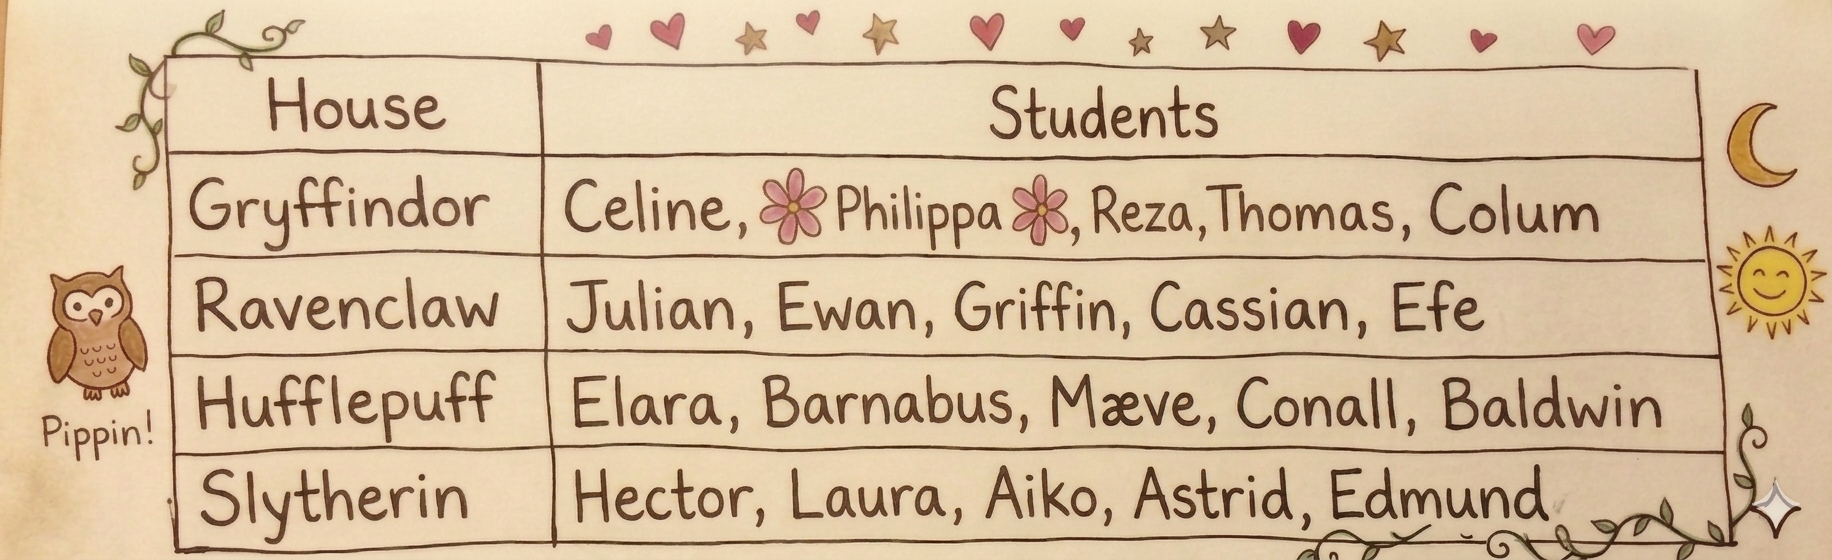
\includegraphics[width=0.75\textwidth]{images/fig_hogwarts_houses_chart_v4.png}
    %\caption{The hare}
    \label{fig_hogwarts_houses_chart}
\end{figure}

\section*{The Feast}

Professor Hepburn pressed the tip of his wand to his throat.

\enquote{Attention!} His amplified voice rolled across the Great Hall like a warm, heavy wave, filling every corner, silencing the last pockets of excited chatter and nervous laughter. The echoes died against the high stone walls, and a hundred faces turned toward him.

The Headmaster waited until the silence was complete. Then he smiled --- a broad, genuine, deeply satisfied smile that creased his entire face.

\enquote{Now then,} he said, his tone dropping to a conversational warmth that somehow carried just as far. \enquote{Now that every last one of you has been sorted into your respective houses --- and I trust the Hat has made no grievous errors this evening, though I confess it has surprised me once or twice ---} a ripple of laughter crossed the hall, \enquote{--- we may proceed to the part of this night that I suspect you have all been waiting for with considerably more enthusiasm than the Sorting itself.}

He paused, letting the anticipation build, his large hands resting on the edge of the high table.

\enquote{The feast.} He said the word with the reverence of a man who meant it. \enquote{And I will confess freely that no one in this hall has been longing for it more than I have. Ten days of ship's biscuits and the galley's best attempts at stew will do that to a man.}

He drew his wand again, gave it a broad, theatrical sweep toward the far end of the hall, and the Great Hall's heavy oak doors swung open with a deep, resonant groan.

Four large rolls of linen entered first. They moved of their own accord, drifting through the open doors in a stately procession, hovering at the height of a man's chest. They were thick and tightly wound, and as each one reached its designated table, it began to unroll --- slowly, deliberately --- the fabric cascading down the length of the oak in a single, continuous motion, the leading edge smoothing itself flat as it advanced.

The tablecloths were extraordinary. Each was minutely embroidered with scenes depicting the history of Hogwarts --- from the four founders laying the first stones to what appeared to be recent events of the current era --- in a style reminiscent of the Bayeux Tapestry\footnote{An embroidered linen cloth, nearly 70 m long and 0.5 m wide, depicting the Norman conquest of England in 1066.}: figures in profile, towers rendered in sharp, flat perspective, battles and ceremonies and feasts stitched in fine, coloured thread against a cream ground. Around and between the scenes, geometric borders and ornamental flourishes carried the colours of each house: green and silver for Slytherin, blue and bronze for Ravenclaw, yellow and black for Hufflepuff, and red and gold for Gryffindor. The stitching was so fine and so densely worked that the linen seemed less like cloth and more like illuminated manuscript laid flat.

\begin{figure}[H]
    \centering
    %\raggedleft
    %\hspace*{8cm}
    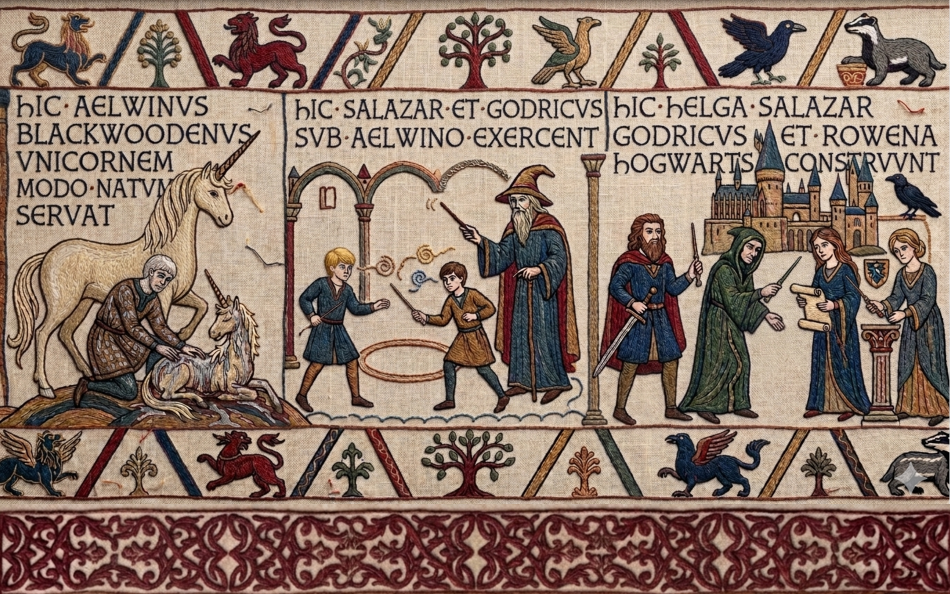
\includegraphics[width=0.99\textwidth]{images/fig_table_cloth_v1.png}
    %\caption{The hare}
    \label{fig_table_cloth}
\end{figure}


Professors Agnes Ravenclaw, Hugh Ligier, and Magnus Grim stood and drew their wands, joining Headmaster Hepburn --- the four heads of house, one for each table. What followed was a piece of choreography so tightly rehearsed that it was impossible to tell where one professor's magic ended and another's began. They moved in perfect synchrony --- four wands tracing arcs and flicks in a continuous, interlocking sequence, the gestures small and precise, the coordination absolute.

Four towering columns of coarse earthenware plates entered through the open doors, stacked impossibly high, each tower leaning at a worrying angle as it drifted across the threshold. A collective intake of breath ran through the first-years. Before a single plate could fall, the towers began to deal. The plates peeled from the bottom of each stack one by one, spinning outward in flat, rapid arcs and settling before each seat like cards being dealt by a croupier --- a sharp, dry click of ceramic on wood, perfectly spaced, perfectly timed.

Then the silverware, the cups, and the chalices --- all distributed with geometric exactness, each piece finding its position in the same instant across all four tables. Ceramic beakers for the spiced ale. Tin chalices for the mulled wine, polished but plain, catching the candlelight in dull, warm flashes. Knives, forks, and spoons followed in neat, glinting lines, dropping into place with a series of rapid, percussive clicks that sounded, for a moment, like applause.

Headmaster Hepburn moved a step forward, and he was smiling. He gave his wand a gentle, looping flick --- a gesture that was almost lazy --- and from beyond the doors came a fluttering, rustling cloud. Napkins. Hundreds of them, folded into the shapes of small birds --- collared doves, by the look of them --- their linen wings held in mid-beat by a stiffening charm. They swept into the hall in a great, wheeling mass, climbing toward the enchanted ceiling before diving toward the tables in playful, spiralling descents.

Thomas saw his coming and raised his hand instinctively to bat it away. The napkin banked sharply, dodged his fingers, looped behind his head, and came at him again from the opposite side. He caught it mid-flight, or thought he did; it wriggled free, fluttered once around his wrist, and tucked itself firmly into his collar with a decisive little flourish. Around the hall, similar small battles were being lost. Colum had given up entirely and sat with his arms crossed, waiting with a look of exasperated dignity as his dove circled him twice before settling. Philippa, who had watched two boys ahead of her fail, simply tilted her chin up and let hers land without resistance; it nestled into place with a satisfied ruffle. A senior student two seats down --- a third-year girl who had not looked up from her cup --- said, without turning, \enquote{Just let them do their job.}

Then the food came.

Great trays entered through the doors in a slow, ponderous procession, each one heavy enough that the magic carrying it seemed to labour under the weight. They settled onto the dressed tables with a deep, wooden exhale.

The centrepiece of each table was a haggis --- split open and steaming, its coarse, peppery smell rising in a thick, savoury column. The filling was dark and crumbled, dense with oats and offal and sharp with the bite of onion and black pepper. Beside each sat a broad, shallow bowl of mashed neeps, pale gold and glistening with butter.

Next came the Scotch broth --- a thick, heavy pottage of pearl barley, mutton, and root vegetables served in deep earthenware bowls. The surface shimmered with fat, and the smell was ancient, elemental --- slow-cooked bone and leek and turnip, the kind of broth that had warmed the Highlands since before the castle's first stone was laid.

Finally, the venison. Whole haunches, roasted dark and lacquered with a glaze of honey and rosemary, the meat pulling apart where the carving knife had already begun its work. The fat had rendered to a thin, crisp bark along the edges, and the juices pooled on the trenchers beneath, soaking into thick rounds of oat bread that served as both plate and sponge.

Behind the food came the drinks. Two sets of tall, narrow-necked jars arranged themselves along the tables. The first set were plain --- unadorned clay, evenly distributed along the full length of each table. The second set, marked with a band of red glaze around the neck, drifted toward the high table where the professors and staff sat, and toward the upper ends of each house table where most of the senior students had gathered.

At the Hufflepuff table, Cecile turned on the bench and caught her sister's eye across the gap between the tables. \enquote{The red jars are for professors, staff, and senior students only,} she said, her voice carrying just enough to reach Celine and Philippa. She held the look for a beat --- the firm, unambiguous gaze of an older sister who did not intend to repeat herself --- then turned back to her own table. Celine reached for the nearest plain jar without comment. Philippa did the same.

The feast began. The noise of the hall rose --- the particular, dense sound of a hundred conversations conducted simultaneously over the scrape of knives and the heavy pouring of drink. The enchanted ceiling above shifted to mirror the sky outside, a deep, clear indigo scattered with early stars.

At the Hufflepuff table, Barnabus Finch set down his beaker of spiced ale and produced a burp of startling resonance. It was not quiet. It carried. Several heads turned. Two Ravenclaw girls covered their mouths. From the Slytherin table, the Bloody Baron's voice cut across the gap like a blade on glass.

\enquote{Mind your manners, boy.}

Barnabus went very still, his rosy cheeks deepening to a shade that might have been mistaken for sunburn. He did not burp again.

A small, ghostly, cackling shape streaked across the hall at speed, barely visible against the tall stonework. It paused --- just long enough --- above a second-year boy at the Ravenclaw table, and a fine dusting of salt rained into his cup. The boy drank, choked, and spat in surprise, his face contorting. \enquote{Peeves!} he sputtered, wiping his mouth furiously. A gleeful laugh echoed off the vaulted ceiling as the shape rocketed toward the far wall and vanished through it. The boy's tablemates offered no sympathy whatsoever; the girl beside him was already laughing so hard that her own drink was in jeopardy.

The feast continued. The trays were emptied and refilled, the broth bowls scraped clean, the venison carved down to the bone. Conversation settled into the easy, lulling rhythm of well-fed contentment. At the Gryffindor table, Celine was explaining something to Colum with animated hand gestures, her earlier nervousness entirely forgotten. Thomas listened with half an ear, his gaze drifting across the hall --- to the green-lit end of the Slytherin table where Laura Orwell sat in silence, to the Ravenclaw bench where Griffin Ollivander appeared to be examining his fork with the same intensity other students reserved for their wands.

As the last of the plates were cleared and the enchanted ceiling deepened toward true night, Headmaster Hepburn rose from his seat. He did not amplify his voice this time. He did not need to; the hall quieted on its own, the conversations thinning and dying like embers.

\enquote{You have eaten well, I hope,} he said, his tone warm and unhurried. \enquote{You have been sorted. You have found your tables and, I hope, begun to find your friends.} He paused, letting his gaze move slowly across the four long tables. \enquote{Now it is time to find your beds.} He clapped his large hands together once, the sound sharp and final against the stone. \enquote{Prefects, lead your houses. First-years, follow closely. The castle is old, and it does not always agree with itself about where the corridors go.} A few tired laughs. \enquote{Sleep well.}

The benches scraped back. The four tables emptied in four directions --- the Gryffindors toward the grand staircase, the Hufflepuffs toward the lower corridors, the Ravenclaws toward the west tower, the Slytherins toward the dungeons. For the first time since the Thames, the group that had formed in Cabin Eleven and grown with every port of call was no longer together. Thomas caught a last glimpse of Cecile's brown hair disappearing down a corridor to the left, of Cassian's tall frame turning right with the Ravenclaws, of Aiko's straight back descending toward the green-lit passage below.

Then they were gone, and the castle had them.

















